To delete a spreadsheet the client will use the \hyperref[sec:message:delete]{delete} 
command, which accepts the \emph{id} of the spreadsheet that is to be deleted. This will 
delete the spreadsheet from the spreadsheet list and all of its history; it will also trigger 
an update for all clients who currently have the spreadsheet \hyperref[sec:message:open]{open}, 
notifying them that the spreadsheet has been deleted.

\begin{figure}[H]
    \begin{center}
        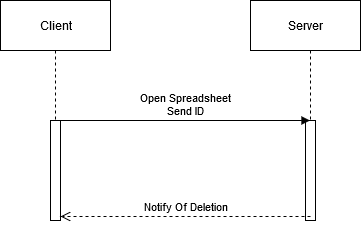
\includegraphics[width=2.5in]{Figures/delete_sprd.png}
        \caption{Deleting a spreadsheet sequence diagram}
    \end{center}
\end{figure}
